%%%%%%%%%%%%%%%%%%%%%%%%%%%%%%%%%%%%%%%%%%%%%%%%%%

\section{\hp}
\label{sec:hephaestus}

\hp~\cite{rbonifacio:sbcars2009} is a
publicly\footnote{\url{https://gitorious.org/hephaestus/pages/Home}}
available product derivation tool~\cite{deelstra:2005}, which receives
contributions from different institutions (Federal University of
Pernambuco, University of S\~{a}o Paulo, University of
Bras\'{i}lia). Initially developed as a proof-of-concept tool for
managing variabilities in use case
scenarios~\cite{rbonifacio:aosd2009}, \hp{} provides a declarative and
executable specification in Haskell of a
compositional~\cite{kastner:2008} and parametric approach for managing
variability in use case scenarios.  Currently, \hp{} supports
variability in different types of artifacts, ranging from business
processes and Simulink models to source code; and it has been used as
the derivation tool in a industrial-strength product
line~\cite{ferreira:2010}.

%%%%%%%%%%%%%%%%%%%%%%%%%%%%%%%%%%%%%%%%%%%%%%%%%%

\subsection{Initial \hp}
\label{S:initial-hp}

For the initial purpose of the tool, the implementation contained the
following entities:

\begin{itemize}
\item Specific data types representing use case models (UCM), feature
  models (FM), and configuration knowledge (CK) model~\cite{gpbook},
  which relates feature expressions in propositional logic to
  transformations that deal with variability in use cases.

\item Specific functions that solve SPL variabilities in use case
  scenarios, by selecting use cases or scenarios from an SPL model,
  composing them, and binding parameters according to specific feature
  configurations.

\item A \texttt{build} function that serves as an interpreter for the
  configuration knowledge and is responsible for building a specific
  product from a given selection of features, i.e., a feature
  configuration (FC).

\item Specific functions providing functionality on use case models.

\end{itemize}

%%%%%%%%%%%%%%%%%%%%%%%%%%%%%%%%%%%%%%%%%%%%%%%%%%

\begin{figure}[t!]
\begin{lstlisting}
type ConfigurationKnowledge = [ConfigurationItem] *'\label{ck-i-1}'*
data ConfigurationItem = ConfigurationItem {
  expression = FeatureExpression,
  transformations = [Transformation]
} *'\label{ck-f-1}'*

build :: FeatureModel *'\label{build-i-1}'*
      -> FeatureConfiguration
      -> ConfigurationKnowledge
      -> SPLModel
      -> InstanceModel
build fm fc ck spl = derive ts spl emptyInstance
where
    ts = concat [transformations c | c <- ck, eval fc (expression c)]
    ucmodel       = splUCM spl
    emptyUCM      = ucmodel { useCases = [] , aspects = [] }
    emptyInstance = InstanceModel fc emptyUCM *'\label{build-f-1}'*

derive [] spl product = product
derive (t:ts) spl product = derive ts spl (t spl product)

type Transformation = SPLModel -> InstanceModel -> InstanceModel *'\label{transf-1}'*

data SPLModel = SPLModel { *'\label{splmodel-i-1}'*
   splFeatureModel :: FeatureModel,
   splUCM :: UseCaseModel
} *'\label{splmodel-f-1}'*

data InstanceModel = InstanceModel { *'\label{instancemodel-i-1}'*
   featureConfiguration :: FeatureConfiguration,
   ucm :: UseCaseModel
} *'\label{instancemodel-f-1}'*

exportProduct :: Path -> InstanceModel -> IO () *'\label{exportP-i-1}'*
exportProduct t product = do
  exportUcmToLatex (t ++ ``/doc.tex'') (ucm product) *'\label{exportP-f-1}'*

exportUcmToLatex = ... -- functionality specific to use case models
\end{lstlisting}
\caption{Code snippet of the initial implementation of \hp}
\label{fig:hp-initial}
\end{figure}

%%%%%%%%%%%%%%%%%%%%%%%%%%%%%%%%%%%%%%%%%%%%%%%%%%

Figure~\ref{fig:hp-initial} presents a code snippet of
the initial implementation of \hp{} including data types related to
configuration knowledge (lines \ref{ck-i-1}-\ref{ck-f-1}) and a
corresponding interpreter (the \texttt{build} function, in lines
\ref{build-i-1}-\ref{build-f-1}), and the signature of the
transformation functions (line \ref{transf-1}). The configuration
knowledge relates the problem space (through a feature expression) to
the solution space (through a list of asset transformations). Each
transformation solves some variation point in the SPL asset base. The
\texttt{build} function has four input artifacts (FM, FC, CK, and SPL)
and generates a product, i.e., an instance of the SPL. The build
process evaluates the rows of the CK, validating each feature
expression according to the FC--- the set of features that
characterizes a given product. If a feature expression of the CK is
true for the given FC, then the corresponding transformations are
applied to the emerging instance. In addition, the code snippet also
shows the initial representation of the data types \texttt{SPLModel}
(lines \ref{splmodel-i-1}-\ref{splmodel-f-1}) and
\texttt{InstanceModel} (lines
\ref{instancemodel-i-1}-\ref{instancemodel-f-1}). Both types collect
assets and group them with the feature model or the feature
configuration, respectively. The build process eliminates all
variability from the \texttt{SPLModel} value and computes the
\texttt{InstanceModel} value. The \texttt{exportProduct} function
(lines \ref{exportP-i-1}-\ref{exportP-f-1}) generates a \LaTeX\
representation of a product-specific use case model.

%%%%%%%%%%%%%%%%%%%%%%%%%%%%%%%%%%%%%%%%%%%%%%%%%%

\subsection{Ecolution of \hp} 
\label{hp-evolution}

In the context of a R\&D project, \hp{} was used as a replacement for
a proprietary tool that was used to manage variabilities in an
industrial-strength product line~\cite{ferreira:2010}. In this
context, \hp{} had to be evolved so that it could manage variability
not only in use case scenarios, but also in higher level requirements
and source code. Variability in source code means here that source
files can be selected for inclusion into the product, triggering
compilation and preprocessing, thereby solve yet more variability
within the source code. We show the configurations for both the
initial release and the evolved releases in
Figure~\ref{fig:hephaestus-conf1a} and
Figure~\ref{fig:hephaestus-conf1b}.

%%%%%%%%%%%%%%%%%%%%%%%%%%%%%%%%%%%%%%%%%%%%%%%%%%

\begin{figure*}[t!]
\begin{center}
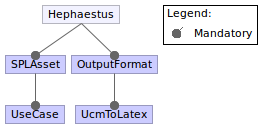
\includegraphics[scale=0.6]{imagens/conf1a-hp.png}
\caption{Configuration of \hp{} in the first release.}
\label{fig:hephaestus-conf1a}
\end{center}
\end{figure*}

%%%%%%%%%%%%%%%%%%%%%%%%%%%%%%%%%%%%%%%%%%%%%%%%%%

\begin{figure*}[t!]
\begin{center}
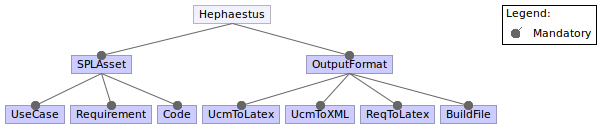
\includegraphics[scale=0.6]{imagens/conf1b-hp.png}
\caption{Configuration of \hp{} in the second release.}
\label{fig:hephaestus-conf1b}
\end{center}
\end{figure*}

%%%%%%%%%%%%%%%%%%%%%%%%%%%%%%%%%%%%%%%%%%%%%%%%%%

Evolution required that new data types and transformations were added
and some of the existing code had to be changed. Precisely, to
introduce support for variability in high-level requirements (or
requirements for short) and source code, the following implementation
and evolution steps were necessary:

\begin{enumerate}[(a)]

\item Implementation of new data types for representing requirements
  and references to source-code assets.

\item Implementation of new parsing and output functions for
  reading/writing requirements and source-code assets into/from \hp.

\item Implementation of new transformations for resolving
  variabilities in requirements and source code.

\item Evolution of the configuration knowledge XML parser so that it
  could recognize the concrete syntax of the new transformations.

\item Evolution of the base product instance used by the \texttt{build}
  function.

\item Evolution of both, \texttt{SPLModel} and \texttt{InstanceModel}
  data types, to collect new assets.

\end{enumerate}

%%%%%%%%%%%%%%%%%%%%%%%%%%%%%%%%%%%%%%%%%%%%%%%%%%

\begin{figure}[t!]
\begin{lstlisting}
data SPLModel = SPLModel { *'\label{splmodel-i-2}'*
   splFeatureModel :: FeatureModel,
   splUCM :: UseCaseModel,
   splReq :: RequirementModel,
   splComponents :: ComponentModel *'\label{splComponents-2}'*
} *'\label{splmodel-f-2}'*

data InstanceModel = InstanceModel { *'\label{instancemodel-i-2}'*
   featureConfiguration :: FeatureConfiguration,
   ucm :: UseCaseModel,
   req :: RequirementModel,
   components :: ComponentModel, *'\label{components-2}'*
   buildEntries :: [PreprocessingDirective], *'\label{buildEntries-2}'*
   preProcessFiles :: [PreprocessingFiles] *'\label{preProcessFiles-2}'*
} *'\label{instancemodel-f-2}'*

build :: FeatureModel -> FeatureConfiguration 
      -> ConfigurationKnowledge -> SPLModel -> InstanceModel
build fm fc ck spl = derive ts spl emptyInstance
where
    ts = concat [transformations c | c <- ck, eval fc (expression c)]
    ucmodel       = splUCM spl
    emptyUCM      = ucmodel { useCases = [] , aspects = [] }  *'\label{emptyInstance-i-2}'*
    emptyReq      = RM { reqs = [] }
    emptyInstance = InstanceModel fc emptyUCM emptyReq [] [] [] *'\label{emptyInstance-f-2}'*

exportProduct :: FilePath -> FilePath -> InstanceModel -> IO ()  *'\label{exportP-i-2}'*
exportProduct s o product = do
  exportUcmToLatex (o ++ ``/doc.tex'') (ucm product)
  exportRequirementsToLatex (o ++ ``/doc.lst'') (req product)
  exportSourceCode s o product  *'\label{exportP-f-2}'*

exportRequirementsToLatex :: FilePath -> RequirementModel -> IO ()
exportSourceCode o rm = ... -- functionality dealing with source code

exportSourceCode :: FilePath -> FilePath -> InstanceModel -> IO ()
exportSourceCode s o p = ... -- functionality dealing with source code
\end{lstlisting}
\caption{\texttt{SPLModel} and \texttt{InstanceModel} data types,
  \texttt{emptyInstance} definition and \texttt{exportProduct}
  function after introducing support for managing variabilities in
  requirements and source code}
\label{fig:spl-model-with-req-and-code}
\end{figure}

%%%%%%%%%%%%%%%%%%%%%%%%%%%%%%%%%%%%%%%%%%%%%%%%%%

The evolution of data types and functions of \hp{}, as described
above, is illustrated in Figure~\ref{fig:spl-model-with-req-and-code}
and Figure~\ref{fig:xml-transformation-parser}. To introduce support
for new types of artifacts, we have to change the \texttt{SPLModel}
data type (lines \ref{splmodel-i-2}-\ref{splmodel-f-2} in
Figure~\ref{fig:spl-model-with-req-and-code}), the
\texttt{InstanceModel} data type (lines
\ref{instancemodel-i-2}-\ref{instancemodel-f-2}), the empty product
definition (lines \ref{emptyInstance-i-2}-\ref{emptyInstance-f-2}),
the \texttt{exportProduct} function (lines
\ref{exportP-i-2}-\ref{exportP-f-2}), and the
\texttt{xml2Transformation} function of the XML parser for
configuration knowledge (Figure~\ref{fig:xml-transformation-parser}).

In contrast, the data types \texttt{ConfigurationKnowledge} and
\texttt{FeatureModel} as well as the \texttt{build} function do not
require any revision, when we introduce variability support for new
types of artifacts.

In particular, evolving \hp{} to support source code variability
(Figure~\ref{fig:spl-model-with-req-and-code}) required a new type of
asset in the \texttt{SPLModel} (\texttt{splComponents}, line
\ref{splComponents-2}). This asset is a list of pairs that relate a
name to the relative path of a source code file. The same type of
asset was also introduced into the \texttt{InstanceModel} (line
\ref{components-2}). Besides that, two other fields were required in
the InstanceModel: (a) \texttt{buildEntries} (line
\ref{buildEntries-2}), which declares pre-processing directives, and
(b) \texttt{preProcessFiles} (line \ref{preProcessFiles-2}), which
declares a list of files that should be pre-processed by a third part
tool. These fields are instantiated when \hp{} builds a product.

%%%%%%%%%%%%%%%%%%%%%%%%%%%%%%%%%%%%%%%%%%%%%%%%%%

\begin{figure}[t!]
\begin{lstlisting}
xml2Transformation :: XmlTransformation -> Parser Transformation
xml2Transformation transformation =
let
  args = ...
  tnsName = xmlTransformationName transformation
in
  case tnsName of
   "selectScenarios" -> Success (selectScenarios args) *'\label{transformations-ucm-i-2}'*
   "selectUseCases" -> Success (selectUseCases args)
   "evaluateAspects" -> Success (evaluateAspects args)
   "bindParameter" -> ...  *'\label{transformations-ucm-f-2}'*
   "selectRequirements" -> ... *'\label{transformations-req-2}'*
   "selectComponents" -> ... *'\label{transformations-code-i-2}'*
   "selectAndMoveComponent" -> ...
   "createBuildEntries" -> ...
   "preprocessFiles" -> ... *'\label{transformations-code-f-2}'*
   _ -> Fail ``...''
\end{lstlisting}
\caption{Code snippet for the XML parser for configuration knowledge}
\label{fig:xml-transformation-parser}
\end{figure}

%%%%%%%%%%%%%%%%%%%%%%%%%%%%%%%%%%%%%%%%%%%%%%%%%%

The code snippet in Figure~\ref{fig:xml-transformation-parser} shows
the revised XML parser for configuration knowledge. The initial
version of \hp{} declared just the first four case statements on the
\texttt{xml2Transformation} function (lines
\ref{transformations-ucm-i-2}-\ref{transformations-ucm-f-2}). The
added \texttt{selectRequirements} transformation (line
\ref{transformations-req-2}) deals with variability in the
requirements models, whereas the remaining transformations (lines
\ref{transformations-code-i-2}-\ref{transformations-code-f-2}) deal
with variability in source code. 

Likewise, \hp{} also provides limited configurability: to obtain a new
version of \hp{} managing variability in only a proper subset of the
types of artifacts currently supported (use cases, requirements,
source code), e.g., a version supporting only source code and use
cases, the change impact is similar to what has been described
previously when extending \hp{} to target new types of artifacts.

%%%%%%%%%%%%%%%%%%%%%%%%%%%%%%%%%%%%%%%%%%%%%%%%%%

\subsection{\hp's `Expression Problem'}
\label{S:xp}

Technically, the evolution scenario demonstrated an extensibility
problem. We had to extend data types and functions to incorporate new
types of artifacts, transformations, and support functionality (e.g., for
exporting). We failed to provide a modular extension; instead, we
ended up revising existing code.

The well-known `Expression Problem'
(EP~\cite{Wadler98,Lopez-HerrejonBC05}) captures this sort of
challenge in a principle manner: \emph{Given a family of data variants
  and a family of operations on the data, how can we design an
  implementation of data and operations such that new variants and new
  operations can be added without revising existing code, while
  possibly also providing some degree of separate compilation, modular
  type checking, and modular reasoning?}

Programming language support for the EP, as discussed below, helps
with modularization so that evolution scenarios, like the one
discussed above, can be potentially carried out without revising
existing code.

Hinze and L\"oh proposed a Haskell extension for open data types and
functions for Haskell~\cite{LoehH06}, which would provide a solution
to the EP in Haskell. The extension allows adding new cases to data
types (i.e., adding cases to `sums', algebraically speaking) and new
equations to functions (i.e., adding cases to a discrimination over a
sum), but it does not deal with additional adaptation patterns
encountered in
Figure~\ref{fig:spl-model-with-req-and-code}. Specifically, the
evolution of \hp{} involved extending `products' as opposed to just
`sums' (see the data types \texttt{SPLModel} and
\texttt{InstanceModel}) and `function compositions' as opposed to just
`case discriminations' (see the the function \texttt{exportProduct}).
Arguably, these adaptation patterns could be eliminated by using a
different data and program design that treats the products instead as
more generic containers, as we discuss in
Section~\ref{sec:implementation}. In either case, open data types and
functions are not available in actual Haskell systems.

L\"ammel and Ostermann proposed a type class-based encoding for
solving the EP in Haskell with relatively established extensions (in
fact, in Haskell~98 for the narrow EP)~\cite{LaemmelO06}. The encoding
overhead is substantial. Data types like \texttt{SPLModel} and
\texttt{InstanceModel} and functions like \texttt{exportProduct} and
\texttt{xml2Transformation} would need to be represented as type
classes, their constructors and equations would give rise to extra
data types and type-class instances, leading to a substantial increase
in code size and a negative impact on comprehensibility, e.g., due to
more complex type-error messages. The approach also fails at the
aforementioned adaptation patterns, which go beyond the EP. More
subtly, the approach also fails at function extension scenarios that
are not readily based on different constructors; see
\texttt{xml2Transformation}, where all equations match on strings.

Ultimately, the domain design of \hpl{} (see
Section~\ref{sec:domainDesign}) leverages a transformational approach
to managing variability with an implementation (see
Section~\ref{sec:implementation}) based on Haskell
\emph{metaprogramming}. The approach readily covers all adaptation
patterns, it directly works with existing Haskell systems, it easily
integrates with feature modeling and configuration, and it enables
bootstrapping of \hpl{}.

%%%%%%%%%%%%%%%%%%%%%%%%%%%%%%%%%%%%%%%%%%%%%%%%%%
